\paragraph{}{
	Le second circuit éléectronique composant le processeur est
	le contrôleur de saut. Son rôle est de mettre à jour \textit{PC}
	en fonction du résultat de l'opération que vient d'effectuer
	l'UAL pour le cycle suivant. Le saut est déterminé en fonction
	des indicateurs que le circuit à en entrée, c'est-à-dire 
	\textit{SF} et \textit{ZF}. Pour celà, on fait un tableau de
	Karnaugh, à la figure \ref{karnaugh_ctrl_saut}.
}

\begin{figure}
	\centering
	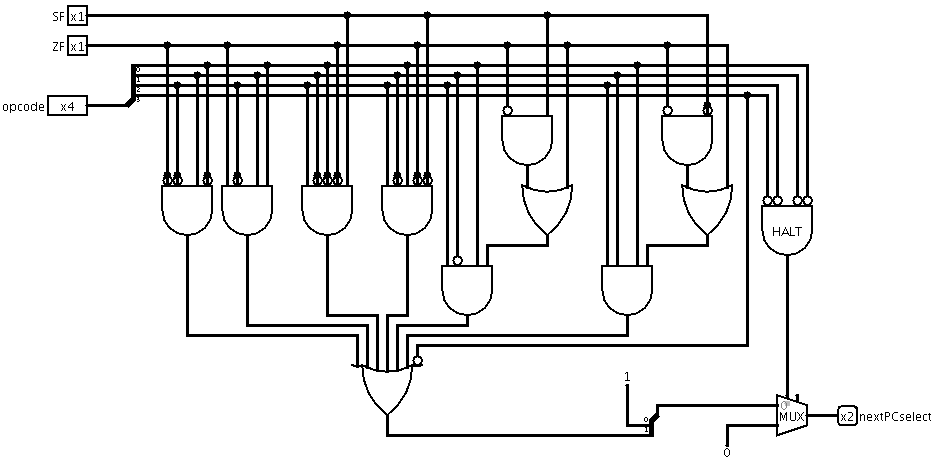
\includegraphics[scale=0.4,origin=c]{circuits/control_saut.png}
	\label{control_saut_circ}
	\caption{Sch\'{e}ma \'{e}lectronique du contr\^{o}leur de sauts}
\end{figure}

\begin{figure}
	\centering
	\begin{tabular}{|c|c|c|c|c|c|}
		\hline 
		O2 & O1 & O0 & ZF & SF & C1 \\ 
		\hline 
		$0$ & $0$ & $1$ & $\times$ & $\times$ & $0$ \\ 
		\hline 
		$0$ & $1$ & $0$ & $0$ & $\times$ & $1$ \\ 
		\hline 
		$0$ & $1$ & $0$ & $0$ & $\times$ & $0$ \\ 
		\hline 
		$0$ & $1$ & $1$ & $1$ & $\times$ & $0$ \\ 
		\hline 
		$0$ & $1$ & $1$ & $1$ & $\times$ & $1$ \\ 
		\hline 
		$1$ & $0$ & $0$ & $0$ & $0$ & $0$ \\ 
		\hline 
		$1$ & $0$ & $0$ & $0$ & $1$ & $1$ \\ 
		\hline 
		$1$ & $0$ & $0$ & $1$ & $0$ & $0$ \\ 
		\hline 
		$1$ & $0$ & $0$ & $1$ & $1$ & $0$ \\ 
		\hline 
		$1$ & $0$ & $1$ & $0$ & $0$ & $1$ \\ 
		\hline 
		$1$ & $0$ & $1$ & $0$ & $1$ & $0$ \\ 
		\hline 
		$1$ & $0$ & $1$ & $1$ & $0$ & $0$ \\ 
		\hline 
		$1$ & $0$ & $1$ & $1$ & $1$ & $0$ \\ 
		\hline 
		$1$ & $1$ & $0$ & $0$ & $0$ & $0$ \\ 
		\hline 
		$1$ & $1$ & $0$ & $0$ & $1$ & $1$ \\ 
		\hline 
		$1$ & $1$ & $0$ & $1$ & $0$ & $1$ \\ 
		\hline 
		$1$ & $1$ & $0$ & $1$ & $1$ & $1$ \\ 
		\hline 
		$1$ & $1$ & $1$ & $0$ & $0$ & $1$ \\ 
		\hline 
		$1$ & $1$ & $1$ & $0$ & $1$ & $0$ \\ 
		\hline 
		$1$ & $1$ & $1$ & $1$ & $0$ & $1$ \\ 
		\hline 
		$1$ & $1$ & $1$ & $1$ & $1$ & $1$ \\ 
		\hline 
	\end{tabular} 
	\label{karnaugh_ctrl_saut}
	\caption{Tableau de Karnaugh du contrôleur de saut}
\end{figure}

\paragraph{}{
	Le schéma électronique du contrôleur de saut est à la figure
	\ref{control_saut_circ}. 
}